\chapter{Arhitectura aplicației}

În mare parte aplicația este construită în jurul unei singure scene folosind $Unity$, arhitectura aplicației depinzând în mare parte de uneltele disponibile în motorul grafic și modul în care acesta funcționează Am încercat să împart căt de mult se poate să împart aplicația în module cu o coeziune căt mai ridicată. De acceea sistemul de instanțiere, generare și amplasare a obiectelor este construit cu principalul scop de a fi modular. Chiar și librăria ce modelează prototipul Markov cu stări invizibile este decuplat de algoritmul de antrenare în sine, putând fi schimbat oricând fără repercursiuni.\par

Aplicația folosește și multe funcții de $callback$ pentru a determina cănd anumite elemente din cadrul jocului ar trebui activate. Spre exemplu cea mai folosită funcție este cea de $OnTriggerEnter$, ce determină cănd un $RigidBody$\footnote{Componenta ce determina daca obiectul este supus motorului de fizica} se intersectează cu un \textit{Box}\textit{Collider}\footnote{Componenta ce determina zona de coliziune a unui obiect}.\par

\begin{lstlisting}[caption=Exemplu de utilizare a functiei OnTriggerEnter]
void OnTriggerEnter(Collider collidingObject){
        if (!this.triggered){
            this.callbackObject.GetComponent<PlatformBuilder>().InstantiatePlatform();
            this.triggered = true;
        }
}
\end{lstlisting}
\par

De asemena $Unity$ dispune de o unealtă foarte utilă numită $Inspector$ ce permite asignarea de referințe a obiectelor din scenă în scripturi, lucru foarte util și eficient atunci cănd este necesară legarea anumitor module. De exemplu $callbackObject$ reprezintă obiectul din scenă de care este atașat codul sursă ce se ocupă de construirea platformelor, numit sugestiv $PlatformBuilder$, din care se apelează funcția $InstantiatePlatform$ destinată acestui scop.\par

\section{Detalii legate de implementarea librăriei}

Cum menționam și anterior pentru implementare am avut nevoie de o librărie ce se ocupă cu calcul numeric. Am folosit $Math.NET$ pentru calculul matriceal și a normelor $L^{2}$, împreună cu structurile speciale $Matrix$ și $Vector$ din cadrul librarie pentru a manipula parametri $\lambda = \{\textbf{A},\textbf{B},\pi\}$ ai modelului.\par

În cadrul librăriei s-au folosit o multitudine de funcții auxiliare ce ajută la normalizare și structurarea mai bună a codului. Mai jost sunt prezentate cele mai importante funcții auxiliare din cadrul acesteia.\par

\begin{lstlisting}[caption=Funcție auxiliara ce realizează normalizarea]
private Matrix<double> Normalize(Matrix<double> target, Vector<double> divisors, string mode){
        Matrix<double> output = Matrix<double>.Build.DenseOfMatrix(target);
        for (int i = 0; i < target.RowCount; ++i){
            for (int j = 0; j < target.ColumnCount; ++j){
                if (mode == "row")
                    output[i, j] /= divisors[i];
                if (mode == "column")
                    output[i, j] /= divisors[j];
            }
        }
        return output;
}
\end{lstlisting}


\begin{lstlisting}[caption=Funcție auxiliara ce construiește matricea de frecvență $C$]
private Matrix<double> GetOccurenceMatrix(List<int> observations){
        Matrix<double> occurences = Matrix<double>.Build.Dense(this.emissionCount, this.emissionCount);
        for (int i = 0; i < observations.Count - 1; ++i){
            occurences[observations[i], observations[i + 1]] += 1;
        }
        return occurences;
}
\end{lstlisting}

\begin{lstlisting}[caption=Funcție auxiliara ce contruieste o matrice cu intrări random]
private void SetRandomMatrix(double[,] matrix){
        double[] divisors = new double[matrix.GetLength(0)];
        double rowMax = 0.0f;
        for (int i = 0; i < matrix.GetLength(0); ++i){
            rowMax = 0;
            for (int j = 0; j < matrix.GetLength(1); ++j){
                matrix[i, j] = Random.Range(0.0f, 100.0f);
                rowMax += matrix[i, j];
            }
            divisors[i] = rowMax;
        }
        Normalize(matrix, divisors);
}
\end{lstlisting}
\clearpage

Legat de aplicarea capitoluilui teoretic, antrenarea este realizată de o singură funcție căreia îi sunt pasați parametri modelului, împreună cu secvența de etichete observate. Funcția aplică ecuațiile discutate în cadrul capitolului de aspecte teoretice, bineînțeles adaptate la limbajul de programare folosit.\par

\begin{lstlisting}[caption=Implementare algoritmului de antrenare a modelului]
public double Train(List<int> observations, double[,] transitionProbabilities, double[,] emissionProbabilities, List<double> pi){
        this.SetEmissionMatrix(emissionProbabilities);
        this.SetTransitionMatrix(transitionProbabilities);
        this.SetDrawProbabilities(pi);
        Matrix<double> previousJoinDistribution = Matrix<double>.Build.Dense(this.emissionCount, this.emissionCount);
        Matrix<double> previousEmission = Matrix<double>.Build.Dense(this.stateCount, this.emissionCount);
        Matrix<double> previousTransition = Matrix<double>.Build.Dense(this.stateCount, this.stateCount);
        Matrix<double> jointDistribution;
        Matrix<double> emissionDelta;
        Matrix<double> transitionDelta;
        Matrix<double> occurenceMatrix = this.GetOccurenceMatrix(observations);
        this.SetMatrixBar();
        this.emissionMatrix = this.emissionMatrix.Transpose();
        previousEmission = previousEmission.Transpose();
        double likelihood = 0.0f;
        for (int i = 0; i < this.maxIterations; ++i){
            jointDistribution = occurenceMatrix.PointwiseDivide(this.emissionMatrix.Multiply(this.transitionMatrix).Multiply(this.emissionMatrix.Transpose()));
            transitionDelta = this.transitionMatrix.PointwiseMultiply(this.emissionMatrix.Transpose().Multiply(jointDistribution).Multiply(this.emissionMatrix));
            emissionDelta = this.emissionMatrix.PointwiseMultiply(jointDistribution.Multiply(this.emissionMatrix).Multiply(this.transitionMatrix.Transpose()).Add(jointDistribution.Transpose().Multiply(this.emissionMatrix).Multiply(this.transitionMatrix)));
            this.transitionMatrix = transitionDelta.Divide(transitionDelta.RowSums().Sum());
            this.emissionMatrix = Normalize(emissionDelta, emissionDelta.ColumnSums(), "column");
            if (this.transitionMatrix.Subtract(previousTransition).L2Norm() < this.epsilon && this.emissionMatrix.Subtract(previousEmission).L2Norm() < this.epsilon && jointDistribution.Subtract(previousJoinDistribution).L2Norm() < this.epsilon)
                break;
            previousEmission = emissionMatrix;
            previousTransition = transitionMatrix;
            previousJoinDistribution = jointDistribution;
        }
        likelihood = GetLikelihood(occurenceMatrix, this.transitionMatrix, this.emissionMatrix.Transpose(), this.emissionMatrix.Multiply(this.transitionMatrix).Multiply(this.emissionMatrix.Transpose()));
        this.transitionMatrix = Normalize(this.transitionMatrix, this.transitionMatrix.RowSums(), "row");
        this.emissionMatrix = this.emissionMatrix.Transpose();
        return likelihood;
}
\end{lstlisting}

Funcția $Train$ descrisă mai sus este folosită în clasa mare denumită sugestiv $HMM$ pentru a antrena modelul. Modul cum funcționează $Unity$ toate clasele ce sunt derivate din $MonoBehaviour$ pot fi atașate pe un obiect din scenă. De accea există un obiect ascuns în scenă ce are atașat toți generatorii, putănd schimba foarte ușor toți parametri modelului chiar din $Inspector$. Din cauza acestui lucru librăria este foarte ușor de preluat și utilizat, aceasta conținând și un modul de salvare/citire a a parametrilor modelului.\par

În continuare se va prezenta o diagramă $UML$ ce descrie librăria și relația dintre componentele ei. Se poate observa că modelul Markov cu stări invizibile poate lucra complet independent de algoritmul de învătare automată.\par

\vspace{10mm}
\begin{figure}[H]
\centering
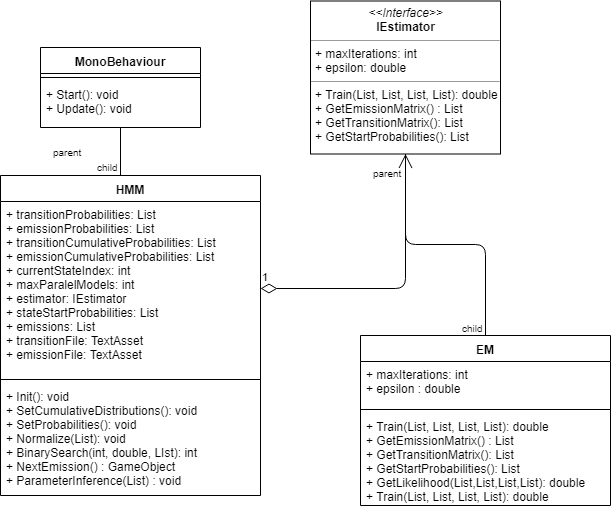
\includegraphics[width=0.8\linewidth]{HMM.png} \par
\caption{Diagrama UML ce modelează libraria de HMM}
\end{figure}

\section{Detalii legate de implementarea sistemului de instanțiere}

\section{Utilizarea librăriei în joc}

\section{Detalii legate de aspectul aplicatiei}

\vspace{10mm}
\begin{figure}[H]
\centering
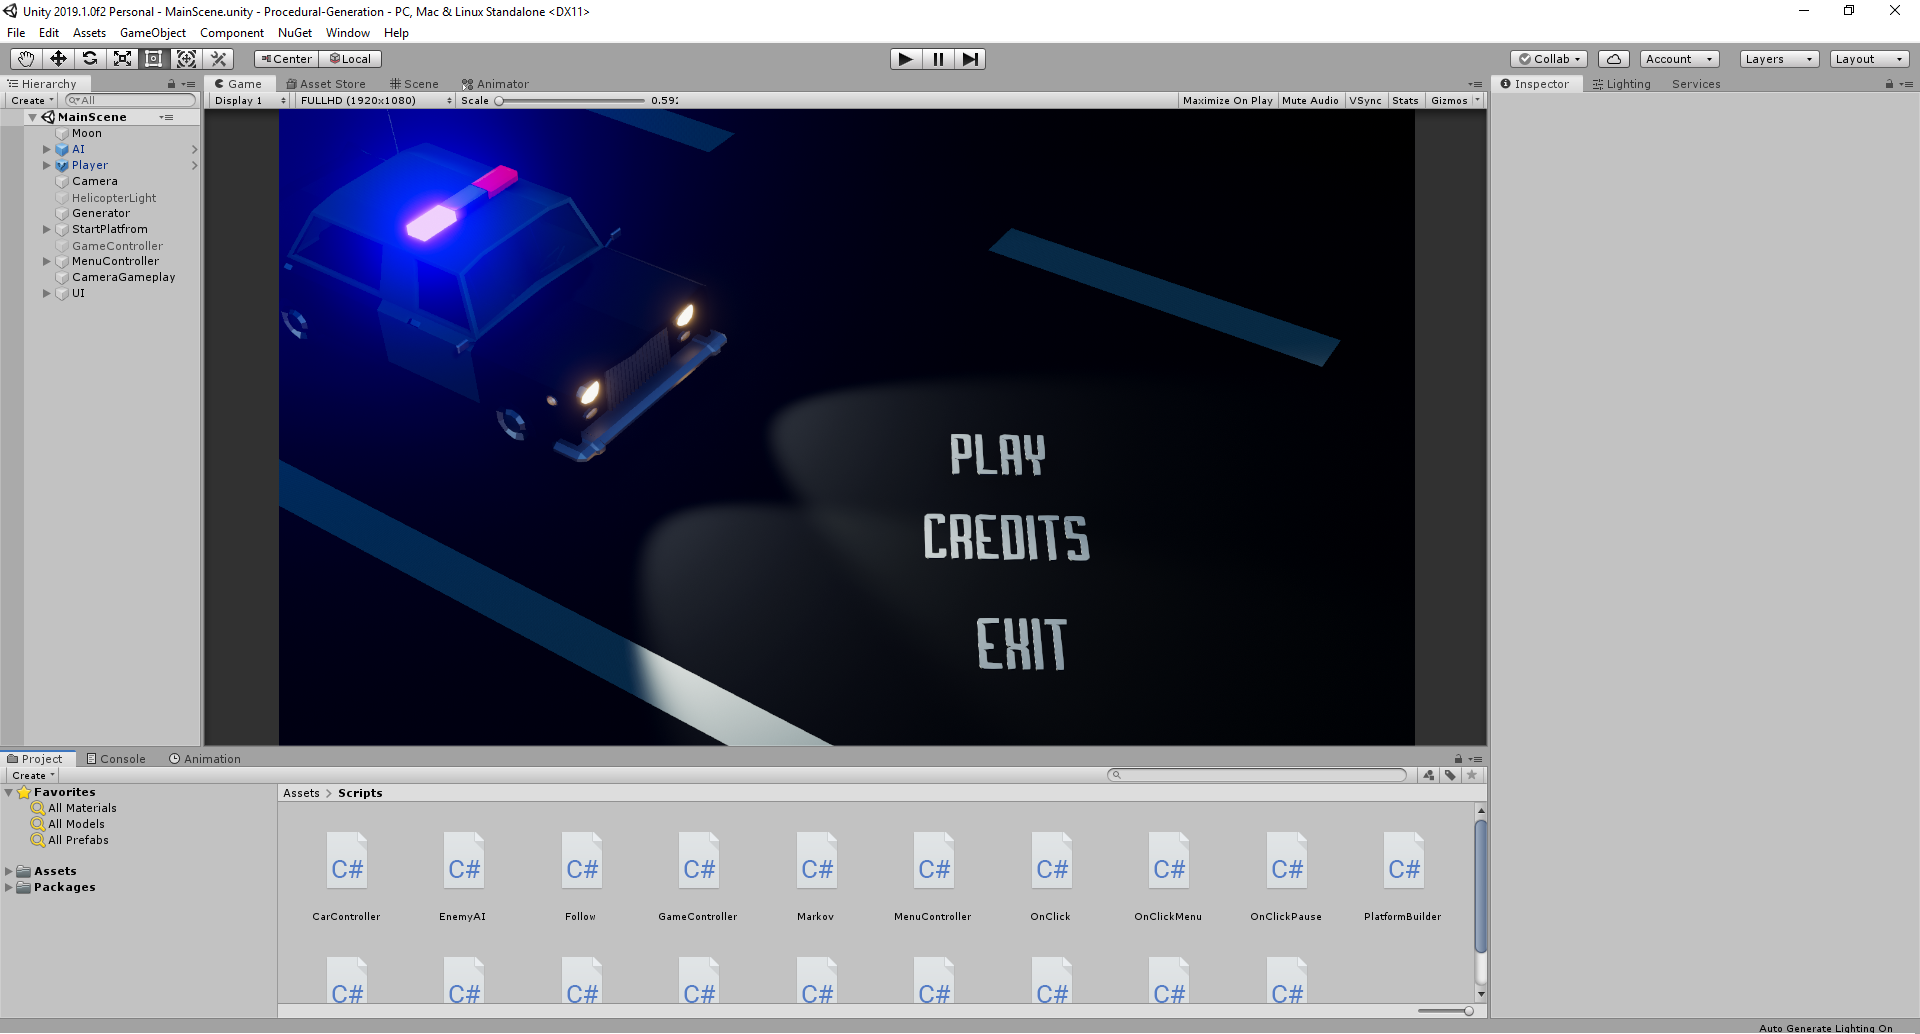
\includegraphics[width=0.65\linewidth]{Unity.png} \par
\caption{Motorul Grafic Unity}
\end{figure}

\section{Structura întregii aplicații}